\providecommand{\tituloDocumento}{Evaluación}
\providecommand{\subtituloDocumento}{Fracciones}

\documentclass{cli-guia}

\begin{document} 
\begin{tcbraster}[enhanced,raster columns=4,raster width=\linewidth,raster column skip=3pt,raster force size=false]
    \begin{caja}[title={\sffamily\scshape\bfseries Nombre},height=35pt,add to width=4.5cm]
    \end{caja}
    \begin{caja}[title={\sffamily\scshape\bfseries Curso},height=35pt,add to width=-1.5cm]
    \end{caja}    
    \begin{caja}[title={\sffamily\scshape\bfseries Puntaje},height=35pt,add to width=-1.5cm]
    \end{caja}
    \begin{caja}[title={\sffamily\scshape\bfseries Nota},height=35pt,add to width=-1.5cm]
    \end{caja}      
\end{tcbraster}
\vspace*{5mm}

{\bfseries Objetivos}
\begin{itemize}
  \item  Transformar (pasar) fracciones impropias a números mixtos y viceversa.
  \item Ubicar fracciones o números mixtos en la recta numérica. 
\end{itemize}
\vspace*{0.2cm}

\begin{problemas}
  \problema ¿Cuál es la diferencia entre una fracción propia y una impropia? [4 p]
  \begin{respuesta}[height=2cm,enlarge top by=5pt]
  \end{respuesta}

  \problema Escribe las siguientes fracciones como número mixto [1 p/u]
  \begin{alternativasgraficas}[]
      \grafica 
      \begin{malla}[height=2cm,enlarge top by=10pt]
        $\dfrac{8}{3}=$
      \end{malla}
      \grafica 
      \begin{malla}[height=2cm,enlarge top by=10pt]
        $\dfrac{24}{5}=$
      \end{malla}
      \grafica 
      \begin{malla}[height=2cm,enlarge top by=10pt]
        $\dfrac{13}{4}=$
      \end{malla}
      \grafica 
      \begin{malla}[height=2cm,enlarge top by=10pt]
        $\dfrac{9}{7}=$
      \end{malla}
      \grafica 
      \begin{malla}[height=2cm,enlarge top by=10pt]
        $\dfrac{15}{7}=$
      \end{malla}
      \grafica 
      \begin{malla}[height=2cm,enlarge top by=10pt]
        $\dfrac{10}{6}=$
      \end{malla}
    \end{alternativasgraficas} 

    

  \problema Escribe los siguientes números mixtos como fracciones impropias [1 p/u]
  \begin{alternativasgraficas}[]
      \grafica 
      \begin{malla}[height=2cm,enlarge top by=10pt]
        $3\dfrac{1}{2}=$
      \end{malla}
      \grafica 
      \begin{malla}[height=2cm,enlarge top by=10pt]
        $1\dfrac{1}{5}=$
      \end{malla}
      \grafica 
      \begin{malla}[height=2cm,enlarge top by=10pt]
        $4\dfrac{1}{3}=$
      \end{malla}
      \grafica 
      \begin{malla}[height=2cm,enlarge top by=10pt]
        $2\dfrac{2}{5}=$
      \end{malla}
      \grafica 
      \begin{malla}[height=2cm,enlarge top by=10pt]
        $2\dfrac{3}{5}=$
      \end{malla}
      \grafica 
      \begin{malla}[height=2cm,enlarge top by=10pt]
        $4\dfrac{12}{17}=$
      \end{malla}
  \end{alternativasgraficas} 


  \problema Ubica en la recta numérica las siguientes fracciones y números mixtos [2 p/u]

  \begin{itemize}[partopsep=0.5cm, itemsep=0.3cm]
    \item $1\dfrac{3}{5}$
    \item $\dfrac{9}{4}$
    \item $\dfrac{14}{3}$
  \end{itemize}

  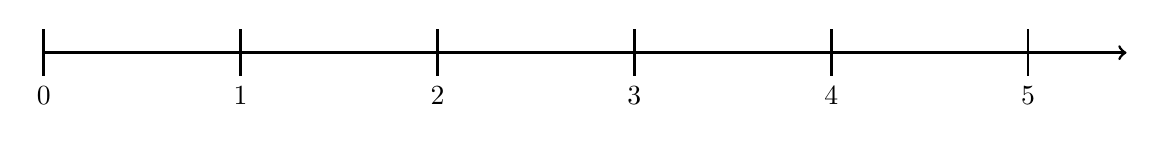
\begin{tikzpicture}[x=2.5cm, line width=1pt]
    \draw [->] (0,0) -- (5.5,0);
    \foreach \x in {0,...,5} {
      \draw (\x,0.3) -- (\x,-0.3) node[below] {\x};
    }
  \end{tikzpicture}

\end{problemas}


% \begin{malla}[height=2cm,enlarge top by=10pt]
% \end{malla}
% \begin{respuesta}[height=1cm,enlarge top by=5pt]
% \end{respuesta}

\end{document}

